\subsection{Architecture and and Platform}\label{sec:architecture}

The architecture of the system are based on multiple individual components which have been implemented
independently consisting on following parts:

\begin{enumerate}
    \item Core API for image processing (computational pipeline) \cite{greenhouseplusplus}
    \item Web API making the core API accessible from network \cite{greenhouseplusplus}
    \item Desktop client in Visual C\# 2019 \cite{greenhouseplusplus}
    \item Web based progressive web app (PWA) allowing network access of the pipeline \cite{greenhouseplusplus:app}
\end{enumerate}

Figure \ref{fig:arch} shows the high level architecture of the entire application ecosystems.

\begin{figure}[H]
    \centering
    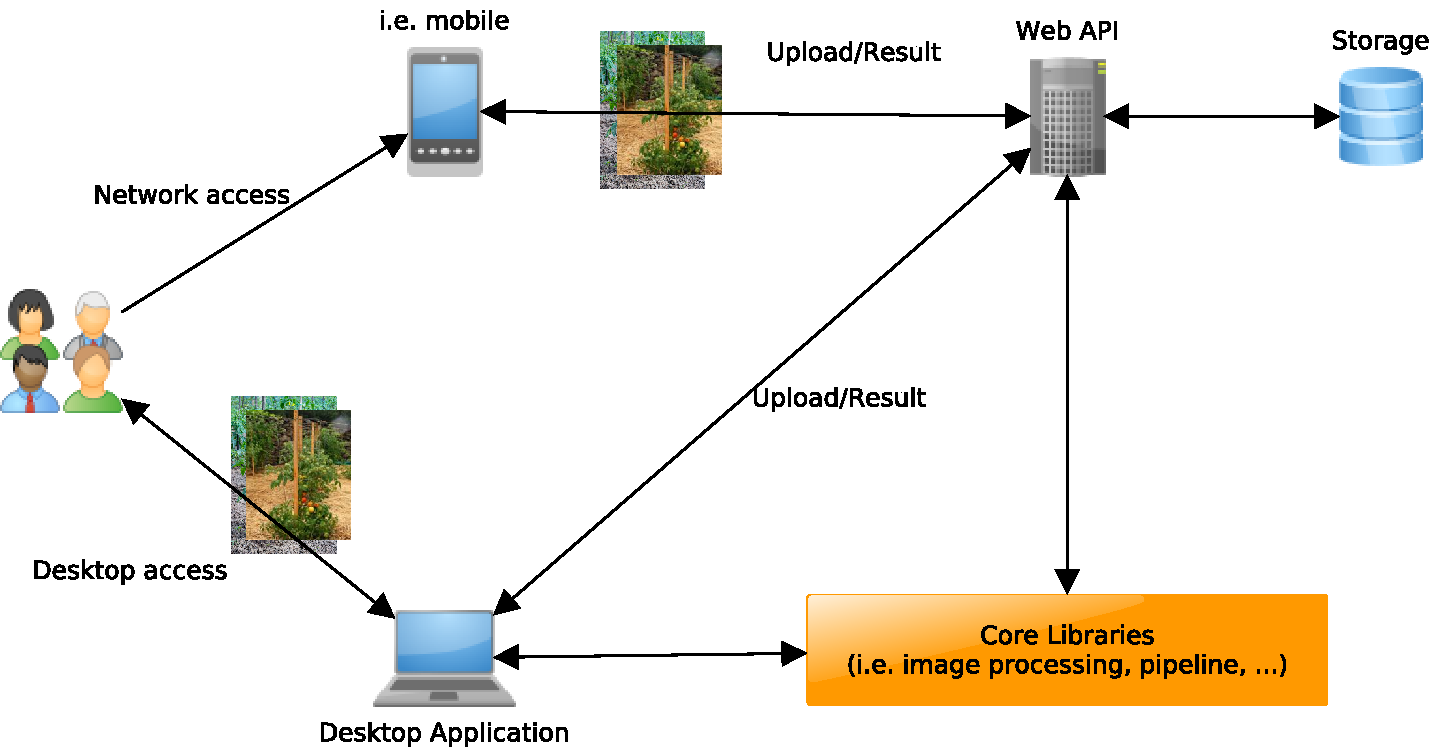
\includegraphics[width=1.0\textwidth]{implementation/architecture.pdf}
    \caption{The pipeline can be accessed by web browser or purely on a Windows desktop.}
    \label{fig:arch}
\end{figure}

The purpose of this architecture is - beside clean implementation and testability - to test a flexible
solution which might also be deployed and used under varying conditions, locations and limited resources.
Figure \ref{fig:desktopclient} show the desktop client conducting the plant tip location and segmentation.

\begin{figure}[H]
    \centering
    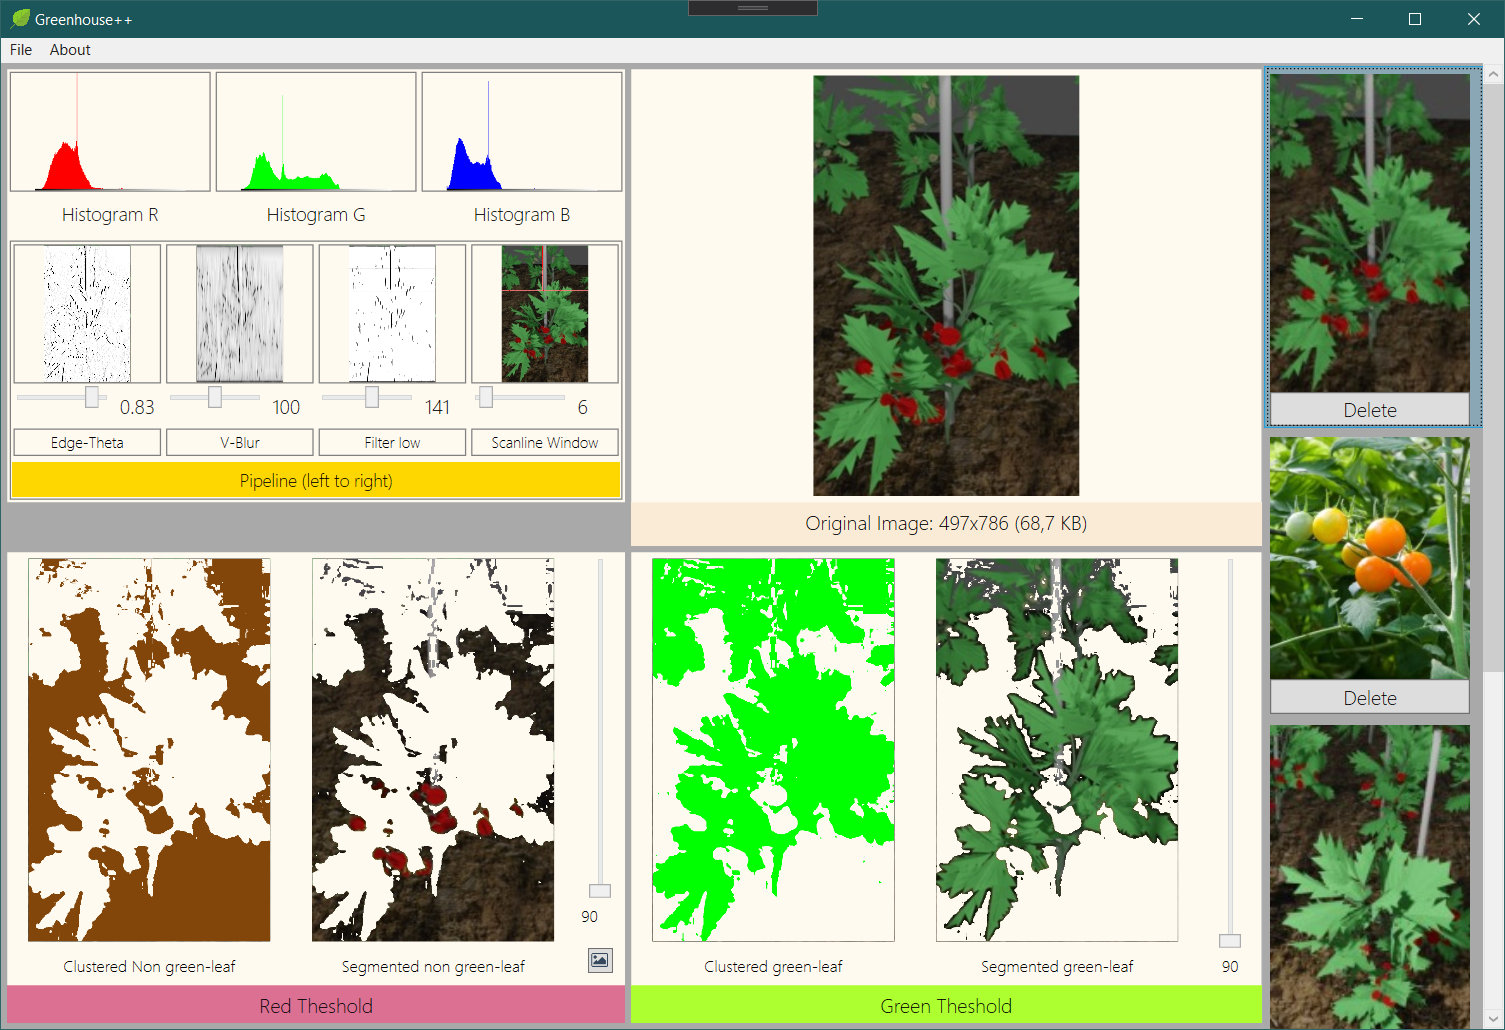
\includegraphics[width=1.0\textwidth]{implementation/greenhouseplusplus-ui.jpg}
    \caption{Visual C\# 2019 Desktop client}
    \label{fig:desktopclient}
\end{figure}

\begin{figure}[H]
    \centering
    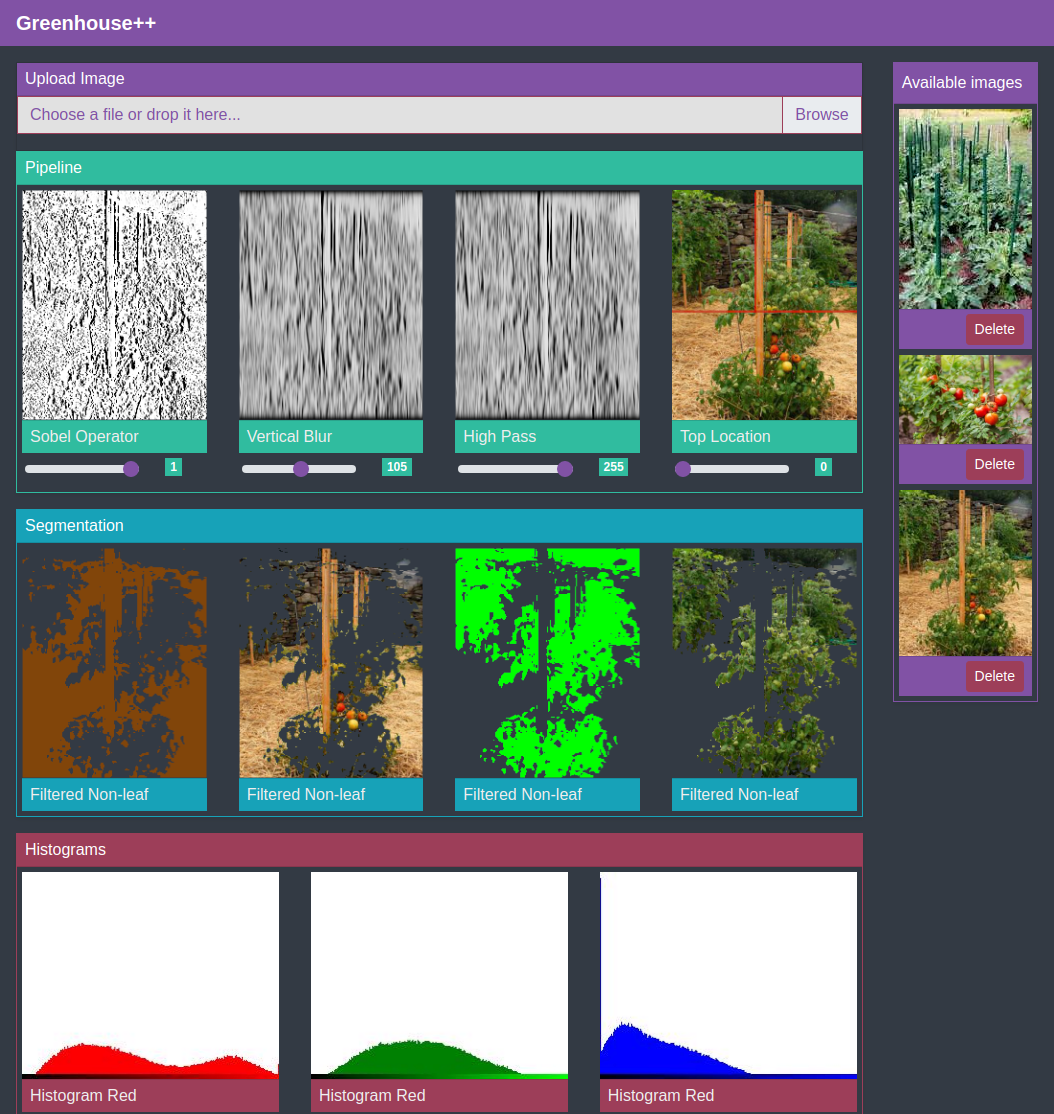
\includegraphics[width=0.7\textwidth]{implementation/web-ui.png}
    \caption{Web based client}
    \label{fig:webclient}
\end{figure}